\documentclass{article}
\usepackage[utf8]{inputenc}
\usepackage[english]{babel}
\usepackage{graphicx}

\DeclareGraphicsExtensions{.pdf,.ps,.png,.jpg}

\newtheorem{theorem}{Theorem}[section]
\newtheorem{corollary}{Corollary}[section]
\newtheorem{lemma}{Lemma}[section]

\author{
  McCaffrey, Caitie\\
  \texttt{Sporty Tights, Inc}
  \and
  Kingsbury, Kyle\\
  \texttt{The SF Eagle}
  \and
  Narula, Neha\\
  \texttt{That's DOCTOR Narula to you!}
}

\title{Distributed Sagas}

\begin{document}

\maketitle

\section{Introduction}

The saga paper outlines a technique for long-lived transactions which provide
atomicity and durability without isolation (what about consistency? Preserved
outside saga scope, not within, right?). In this work, we generalize sagas to
a distributed system, where processes communicate via an asynchronous network,
and discover new constraints on saga sub-transactions.

We are especially interested in the problem of writing sagas which interact with
*third-party services*, where we control the Saga Execution Coordinator (SEC)
and its storage, but not the downstream Transaction Execution Coordinators
(TECs) themselves. Communication between the SEC and TEC(s) takes place over an
asynchronous network (e.g. TCP) which is allowed to drop, delay, or reorder
messages, but not to duplicate them.

We assume a high-availability SEC service running on multiple nodes for
fault-tolerance, where multiple SECs may run concurrently. They coordinate
their actions through a linearizable data store, which ensures Saga
transactions proceed sequentially.

\section{The Saga Execution Coordinator}

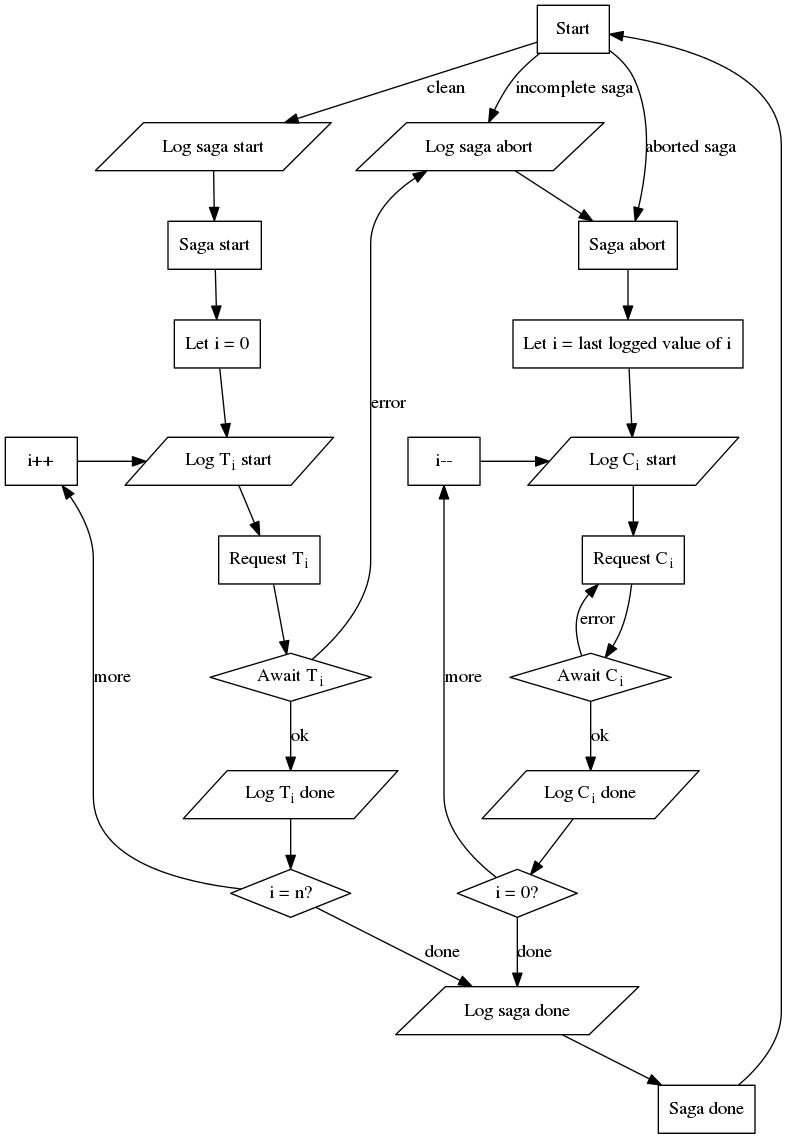
\includegraphics[width=\linewidth]{flow}

\section{Ordering}

\begin{lemma}
I got nothing.
\end{lemma}

\section{Roll-forward}

\section{Rollback}

\end{document}
